% small.tex
\documentclass{beamer}
\usetheme{default}
\usepackage{amsmath, amsfonts, amssymb, amsthm, pstricks, pgf,color,tikz}
\usetikzlibrary{arrows,shapes}


% shared
\newenvironment{frcseries}{\fontfamily{frc}\selectfont}{}
\newcommand{\textfrc}[1]{{\frcseries#1}}
\newcommand{\mathfrc}[1]{\raisebox{-0.8mm}{\text{\textfrc{\small #1}}}\hspace{0.4mm}}
\newcommand{\eqn}[1]{\begin{align*}
#1
\end{align*}}
\newcommand{\eqnl}[2]{\begin{align} \label{#1}
#2
\end{align}}
\newcommand{\vect}[1]{\boldsymbol{\mathbf{#1}}}
\newcommand{\degree}[1]{${#1}^{\circ}$}
\newcommand{\highlight}{ \rowcolor{lightgrass} }
\newcommand{\script}[1]{\mathcal{#1}}
\newcommand{\bl}{\big\{}
\newcommand{\br}{\big\}}
\newcommand{\Bl}{\Big\{}
\newcommand{\Br}{\Big\}}
\newcommand{\argmax}{\operatornamewithlimits{argmax}}
\newcommand{\eqnset}[4]{
\[ #1 = #2 \left\{ \begin{array}{#3}
        #4
\end{array} \right. \] 
}
\definecolor{lemonchiffon}{rgb}{1, .98, .80}
\definecolor{lightgrass}{rgb}{.89, 1, .87}
\newcommand{\clr}[2]{{\color{#1}{#2}}}
\newcommand{\indicator}{\mathbf{1}}
\newcommand{\leftlbl}[1]{\mbox{#1} \;\;\;\;\;\;}
\newcommand{\eqnsep}{,\;\;\;\;\;\;\;\;}


% custom
\newcommand{\afe}{\frac{\alpha}{Fe}}
\newcommand{\feh}{\frac{Fe}{H}}
\newcommand{\vz}{\vect{z}}
\newcommand{\vx}{\vect{x}}
\newcommand{\vy}{\vect{y}}
\newcommand{\vp}{\vect{\pi}}
\newcommand{\vph}{\hat{\vect{\pi}}}
\newcommand{\vpmle}{\hat{\vect{\pi}}_\text{MLE}}
\newcommand{\sumn}{\sum^n_{i=1}}
\newcommand{\summ}{\sum^m_{j=1}}
\newcommand{\summo}{\sum^{m-1}_{j=1}}
\newcommand{\sumg}{\sum^g_{j=1}}
\newcommand{\sumk}{\sum^m_{k=1}}
\newcommand{\fab}{f_j}

\newcommand{\vpg}{\vp^{\prime}}
\newcommand{\vpgh}{\hat{\vp}^{\prime}}
\newcommand{\llp}{\mathfrc{l}(\vect{\pi})}
\newcommand{\llpph}{\mathfrc{l}(\vpgh)}
\newcommand{\llpp}{\mathfrc{l}(\vpg)}




\begin{document}
% For every picture that defines or uses external nodes, you'll have to
% apply the 'remember picture' style. To avoid some typing, we'll apply
% the style to all pictures.
\tikzstyle{every picture}+=[remember picture]

% By default all math in TikZ nodes are set in inline mode. Change this to
% displaystyle so that we don't get small fractions.
\everymath{\displaystyle}







\begin{frame}[shrink]{A generative finite mixture model}
	
	\alert{hello}
	
	\structure{hello}
	
	\pgfputat{\pgfxy(0,-6.5)}{\pgfbox[left,base]{\pgfimage[width=\textwidth]{denstoobs}}}
	
	\begin{itemize}
		\item \clr{red}{a}bc
	\end{itemize}
	
	\eqn{
		\Bigg[\feh,\afe\Bigg]_{i=1}^{N} \text{i.i.d} \sim f(\alert{x},\structure{y}) = \sum^m_{j=1} \pi_j f_j(x,y)
	}
	
\end{frame}




\begin{frame}{Rigid body dynamics}
	
	\tikzstyle{na} = [baseline=-.5ex]
			
			A modest attempt at using PGF/TikZ. \\
		Green's Theorem: \\
		\begin{itemize}
		\item
		Curl \tikz\node[fill=yellow!20,draw,circle] (n4){};
		\item
		Divergence \tikz\node[fill=green!20,draw,circle] (n2){};
		\end{itemize}
		\begin{equation}
		\oint_{\tikz[baseline]{\node[fill=red!20,anchor=base] (t1) {$\partial D$};}} \,
		\tikz[baseline]{\node[fill=green!20,anchor=base] (t2) {$F\cdot ds$};}
		\ = \
		\int\int_{\tikz[baseline]{\node[fill=blue!20,anchor=base] (t3) {$D$};}} \,(
		\tikz[baseline]{\node[fill=yellow!20,anchor=base] (t4) {$\nabla \times F$};})\cdot k \,dA
		\end{equation}
		\begin{itemize}
		\item
		Boundary of Region \tikz\node[fill=red!20,draw,circle] (n1){};
		\item
		Region \tikz\node[fill=blue!20,draw,circle] (n3){};
		\end{itemize}
		\begin{tikzpicture}[overlay]
		\path[->] (n1) edge [out=90, in=-90] (t1);
		\path[->] (n2) edge [bend left] (t2);
		\path[->] (n3) edge [out=0, in=-90] (t3);
		\path[->] (n4) edge [out=0, in=90] (t4);
		\end{tikzpicture}
	\end{frame}








%%%%%%%%%%%%%%%%%%%%%%%%%%%%%%%%%%%%%%%%%%%%%%%%%%%%%%%%%%%%%%%
%%%%%%%%%%%%%%%%%%%%%%%%%%%%%%%%%%%%%%%%%%%%%%%%%%%%%%%%%%%%%%%
\begin{frame}{A generative finite mixture model}
	
	
		
	\begin{figure}
			\begin{center}
				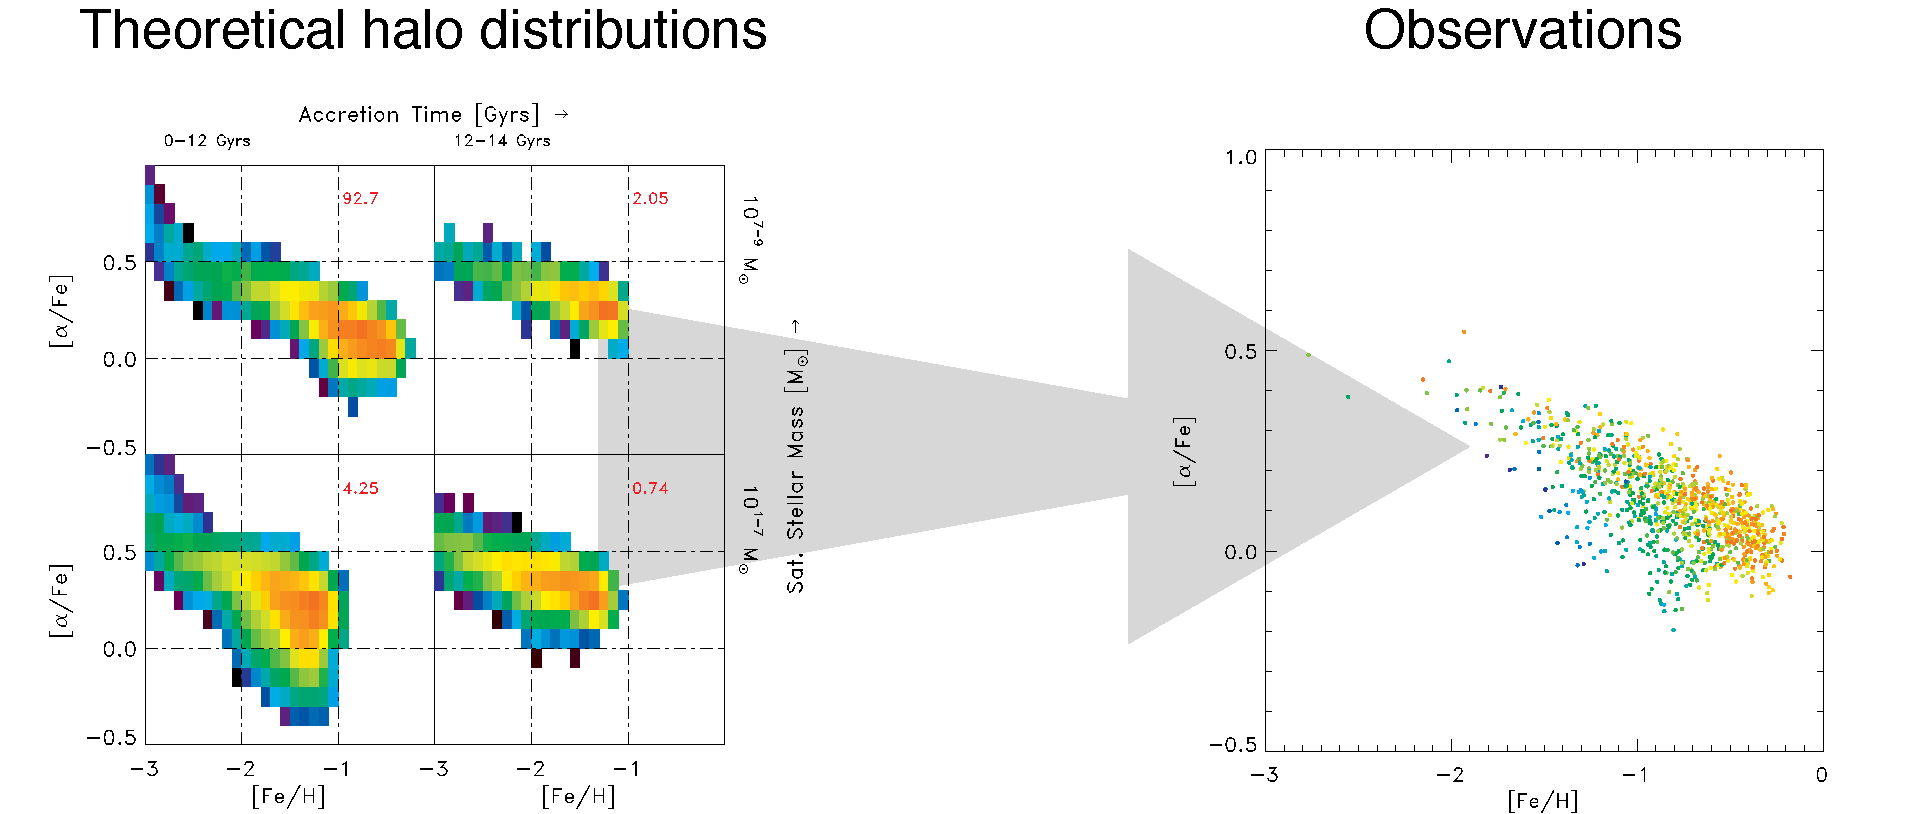
\includegraphics[scale=0.31]{denstoobs.pdf}
			\end{center}
	\end{figure}
	
	\vspace{-8mm}
	
	\eqn{
		\Bigg[\feh,\afe\Bigg]_{i=1}^{N} \text{i.i.d} \sim f(x,y) = \sum^m_{j=1} \pi_j f_j(x,y)
	}
	
	\begin{center}
		Where the mixing proportions, $\vp$, give the formation history.
	\end{center}
	
\end{frame}
%---------------------------------------------------------------------------------------------------------------------------------------------------------------------------
\begin{frame}[shrink]{A generative finite mixture model}
	
	\begin{itemize}
		
		\item each observed point comes from one of $m$ mixture components (pictured)
		\item we propose a generative model in the form of a finite mixture model
		\item since each mixture component has an associated mass and accretion time range, the formation history is specified if we know what percentage of observations come from each mixture component
		\item our goal, then, is to determine the mixing proportions, $\vp$
	\end{itemize}
	
\end{frame}







%%%%%%%%%%%%%%%%%%%%%%%%%%%%%%%%%%%%%%%%%%%%%%%%%%%%%%%%%%%%%%%
%%%%%%%%%%%%%%%%%%%%%%%%%%%%%%%%%%%%%%%%%%%%%%%%%%%%%%%%%%%%%%%
\begin{frame}{Model definition}
	
	\eqn{
		\leftlbl{Let} x=\afe \eqnsep y=\feh
	 }
	
	Given $m$ mixture components, we propose that the density from which observations are generated is
	
	\begin{equation}
		f(x,y) = \sum^m_{j=1}
		\tikz[baseline]{\node[fill=blue!20,anchor=base] (t3) {$\pi_j$};}
		\tikz[baseline]{\node[fill=red!20,anchor=base] (t4) {$f_j(x,y)$};}
	\end{equation}
	\begin{itemize}
		\item
		Mixing proportion \tikz\node[fill=blue!20,draw,circle] (n3){};
		\item
		Mixture component $j$ \tikz\node[fill=red!20,draw,circle] (n4){};
	\end{itemize}
		
	\begin{tikzpicture}[overlay]
		\path[->] (n3) edge [out=0, in=-90] (t3);
		\path[->] (n4) edge [out=0, in=-90] (t4);
	\end{tikzpicture}
	
	
	
	
	
	
	\eqn{
		\leftlbl{where} \sum^m_{j=1} \pi_j = 1 \eqnsep   \pi_j \geq 0  \eqnsep   j=1,\ldots,m
	 }
	
\end{frame}
%---------------------------------------------------------------------------------------------------------------------------------------------------------------------------
\begin{frame}[shrink]{Definitions}
	
	\begin{itemize}
		\item For notational simplicity, x=$\afe$ and y=$\feh$
		\item Formally, given m mixture components, the density from which all observations are drawn is as shown
		\item The mixing proportions, $\vp$ must be non-negative, and sum to 1
	\end{itemize}
	
\end{frame}

















%%%%%%%%%%%%%%%%%%%%%%%%%%%%%%%%%%%%%%%%%%%%%%%%%%%%%%%%%%%%%%%
%%%%%%%%%%%%%%%%%%%%%%%%%%%%%%%%%%%%%%%%%%%%%%%%%%%%%%%%%%%%%%%
\begin{frame}{Estimating the mixing proportions $\vect{\pi}$}
	
	To estimate the mixing proportions, we can use a maximum likelihood approach
	\eqn{
		\vph_{\text{MLE}} &= \argmax_{\vp} L(\vect{\pi})
	}
	
	
	
	\eqn{
		\leftlbl{where} \script{L}(\vect{\pi}) &= \sumn \log \Big( \summ \pi_j \fab(x_i,y_i)  \Big)
	}
	
	Unfortunately the standard MLE procedure for estimating $\vp$ is intractable with this likelihood.\newline
	
	Expectation Maximization (EM) algorithm to the rescue!
	
	
	
\end{frame}
%---------------------------------------------------------------------------------------------------------------------------------------------------------------------------
\begin{frame}[shrink]{Estimating the mixing proportions $\vect{\pi}$}
	
	\begin{itemize}
		\item hi
	\end{itemize}
	
\end{frame}

















%%%%%%%%%%%%%%%%%%%%%%%%%%%%%%%%%%%%%%%%%%%%%%%%%%%%%%%%%%%%%%%
%%%%%%%%%%%%%%%%%%%%%%%%%%%%%%%%%%%%%%%%%%%%%%%%%%%%%%%%%%%%%%%
\begin{frame}{Expectation Maximization}
	
	Suppose we knew which mixture component $f_j$ each observation came from:
	
	\eqnset{z_{ij} = \indicator(x_i,y_i \sim f_j) }{}{ll}{
		1			& (x_i,y_i) \sim f_j 		\\
		0		& \text{otherwise}
	}
	
	The log likelihood can then be expressed as
	
	\eqn{
		\llp &= \sumn \summ z_{ij}  \log \bl \pi_j  \fab(x_i,y_i) \br
	}
	
	The addition of the latent variable $\vect{z}$ actually makes things easier because it is easily differentiable in $\vp$.
	
\end{frame}
%---------------------------------------------------------------------------------------------------------------------------------------------------------------------------
\begin{frame}[shrink]{Expectation Maximization}
	
	\begin{itemize}
		\item Suppose we knew which mixture component $f_j$ each observation came from
		\item Then we could construct a latent indicator variable, $z_{ij}$, which is 1 if point $i$ comes from mixture component $j$, and 0 otherwise
		\item The log like then becomes
		\item Since we're supposing that we know $z_{ij}$, it's trivial to differentiate this log likelihood with respect to $\vph$
		\item 
	\end{itemize}
	
\end{frame}










%%%%%%%%%%%%%%%%%%%%%%%%%%%%%%%%%%%%%%%%%%%%%%%%%%%%%%%%%%%%%%%
%%%%%%%%%%%%%%%%%%%%%%%%%%%%%%%%%%%%%%%%%%%%%%%%%%%%%%%%%%%%%%%
\begin{frame}{Estimating $\vph$ using expectation maximization}
	
	We don't know $\vect{z}$, so we replace $\vect{z}$ with the expected value of $\vect{z}$, conditioned on the data and the last known $\vph$:
	
	%Expectation Maximization replaces the unobservable $\vect{z}$ with the expected value of $\vect{z}$, conditional on the data
	
	\eqn{
		\vph^{(t)} &= \argmax_{\vp} \mathbb{E}\Big[\llp \big| \vx,\vy,\vph^{(t-1)} \Big]   
	}
	
	Starting with some random initial value for $\vph^{(0)}$, we iteratively
	
	\begin{itemize}
		\item Find the expected value of $\llp$ using the current expected values of the latent variable $\vect{z}$
		\item Set $\vph^{(t)}$ to the $\argmax_{\vp}$ of this expectation, which is simple to compute
	\end{itemize}
	
	And repeat until $\llp$ stabilizes to a range  $< 10^{-4}$
	
	
	
\end{frame}
%---------------------------------------------------------------------------------------------------------------------------------------------------------------------------
\begin{frame}[shrink]{Estimating the mixing proportions $\vect{\pi}$}
	
	\begin{itemize}
		\item We don't know $\vect{z}$, so we replace $\vect{z}$ with the expected value of $\vect{z}$, conditioned on the data and the last known $\vph$:
		\item 
		\item the true likelihood is increasing in each iteration
	\end{itemize}
	
\end{frame}








%%%%%%%%%%%%%%%%%%%%%%%%%%%%%%%%%%%%%%%%%%%%%%%%%%%%%%%%%%%%%%%
%%%%%%%%%%%%%%%%%%%%%%%%%%%%%%%%%%%%%%%%%%%%%%%%%%%%%%%%%%%%%%%
\begin{frame}{Find the expected value of $L(\vect{\pi})$ using the current expected value of the latent variable}
	
	The expected value of $\llp$, with respect to the conditional distribution of $\vect{z}$, given observed data and $\vp^{(t-1)}$ is
	
	\eqn{
		\mathbb{E}_{\vp}\Big[\llp \big| \vx,\vy \Big] &= \sumn \summ \mathbb{E}_{\vp}\big[z_{ij}|x_i,y_i\big] \bl \log \fab(x_i,y_i) + \log \pi_j  \br
	}
	
	Since $z_{ij}$ is an indicator, its expected value is simply the probability that data point $i$ comes from model $j$
	\eqn{
		\mathbb{E}_{\vp}\Big[  z_{ij} | x_i, y_i \Big]	&= \text{Pr}_{\vp}(z_{ij}|x_i,y_i)	\\
										&= \frac{p(x_i,y_i|z_{ij}=1)p(z_{ij}=1)}{p(x_i,y_i)}	\\
										&=  \frac{\pi_j \fab(x_i,y_i)  }{\summ \pi_j \fab(x_i,y_i)}
	}
\end{frame}
%---------------------------------------------------------------------------------------------------------------------------------------------------------------------------
\begin{frame}[shrink]{Find the expected value of $L(\vect{\pi})$ using the current expected value of the latent variable}
	
	\begin{itemize}
		\item cond prob
	\end{itemize}
	
\end{frame}














%%%%%%%%%%%%%%%%%%%%%%%%%%%%%%%%%%%%%%%%%%%%%%%%%%%%%%%%%%%%%%%
%%%%%%%%%%%%%%%%%%%%%%%%%%%%%%%%%%%%%%%%%%%%%%%%%%%%%%%%%%%%%%%
\begin{frame}{Find the $\argmax_{\vp}$ of this expectation}
	
		
	Now that we have the expected value of $\llp$ with respect to the conditional distribution of $\vect{z}$, we need only evaluate
	
	
	\eqn{
		\vph^{(t)} &= \argmax_{\vp} \mathbb{E}\Big[\llp \big| \vx,\vy,\vph^{(t-1)} \Big]   
	}
	
	
	Which can be analytically specified, at each time $t$, as:
	
	\eqn{
		\hat{\pi}^{(t)}_k  = \frac{\sumn w^{(t-1)}_{ij}}{n}
	}
	
	\eqn{
		\leftlbl{where} w^{(t+1)}_{ij} = \frac{\pi^{(t)}_{j} \fab(x_i,y_i)}{\sumk \pi^{(t)}_{k}f_k(x_i,y_i)}	
	}
	

	
\end{frame}
%---------------------------------------------------------------------------------------------------------------------------------------------------------------------------
\begin{frame}[shrink]{Find the $\argmax_{\vp}$ of this expectation}
	
	\begin{itemize}
		\item Note how simple this is to compute
	\end{itemize}
	
\end{frame}





















%%%%%%%%%%%%%%%%%%%%%%%%%%%%%%%%%%%%%%%%%%%%%%%%%%%%%%%%%%%%%%%
%%%%%%%%%%%%%%%%%%%%%%%%%%%%%%%%%%%%%%%%%%%%%%%%%%%%%%%%%%%%%%%
\begin{frame}{Simulations}
	
	
	
	
	\begin{itemize}
		\item Generated observations from one halo and multiple halos
		
		\item Used a 5x5 grid ($m=25$), and several 2x2 grids ($m=4$)
		\begin{itemize}
			\item 5x5 grid did not work for some halo realizations
			\item 2x2 grid reliably converged on the correct mixing proportions
		\end{itemize}
	\end{itemize}
	
	
	
	\begin{figure}
			\begin{center}
				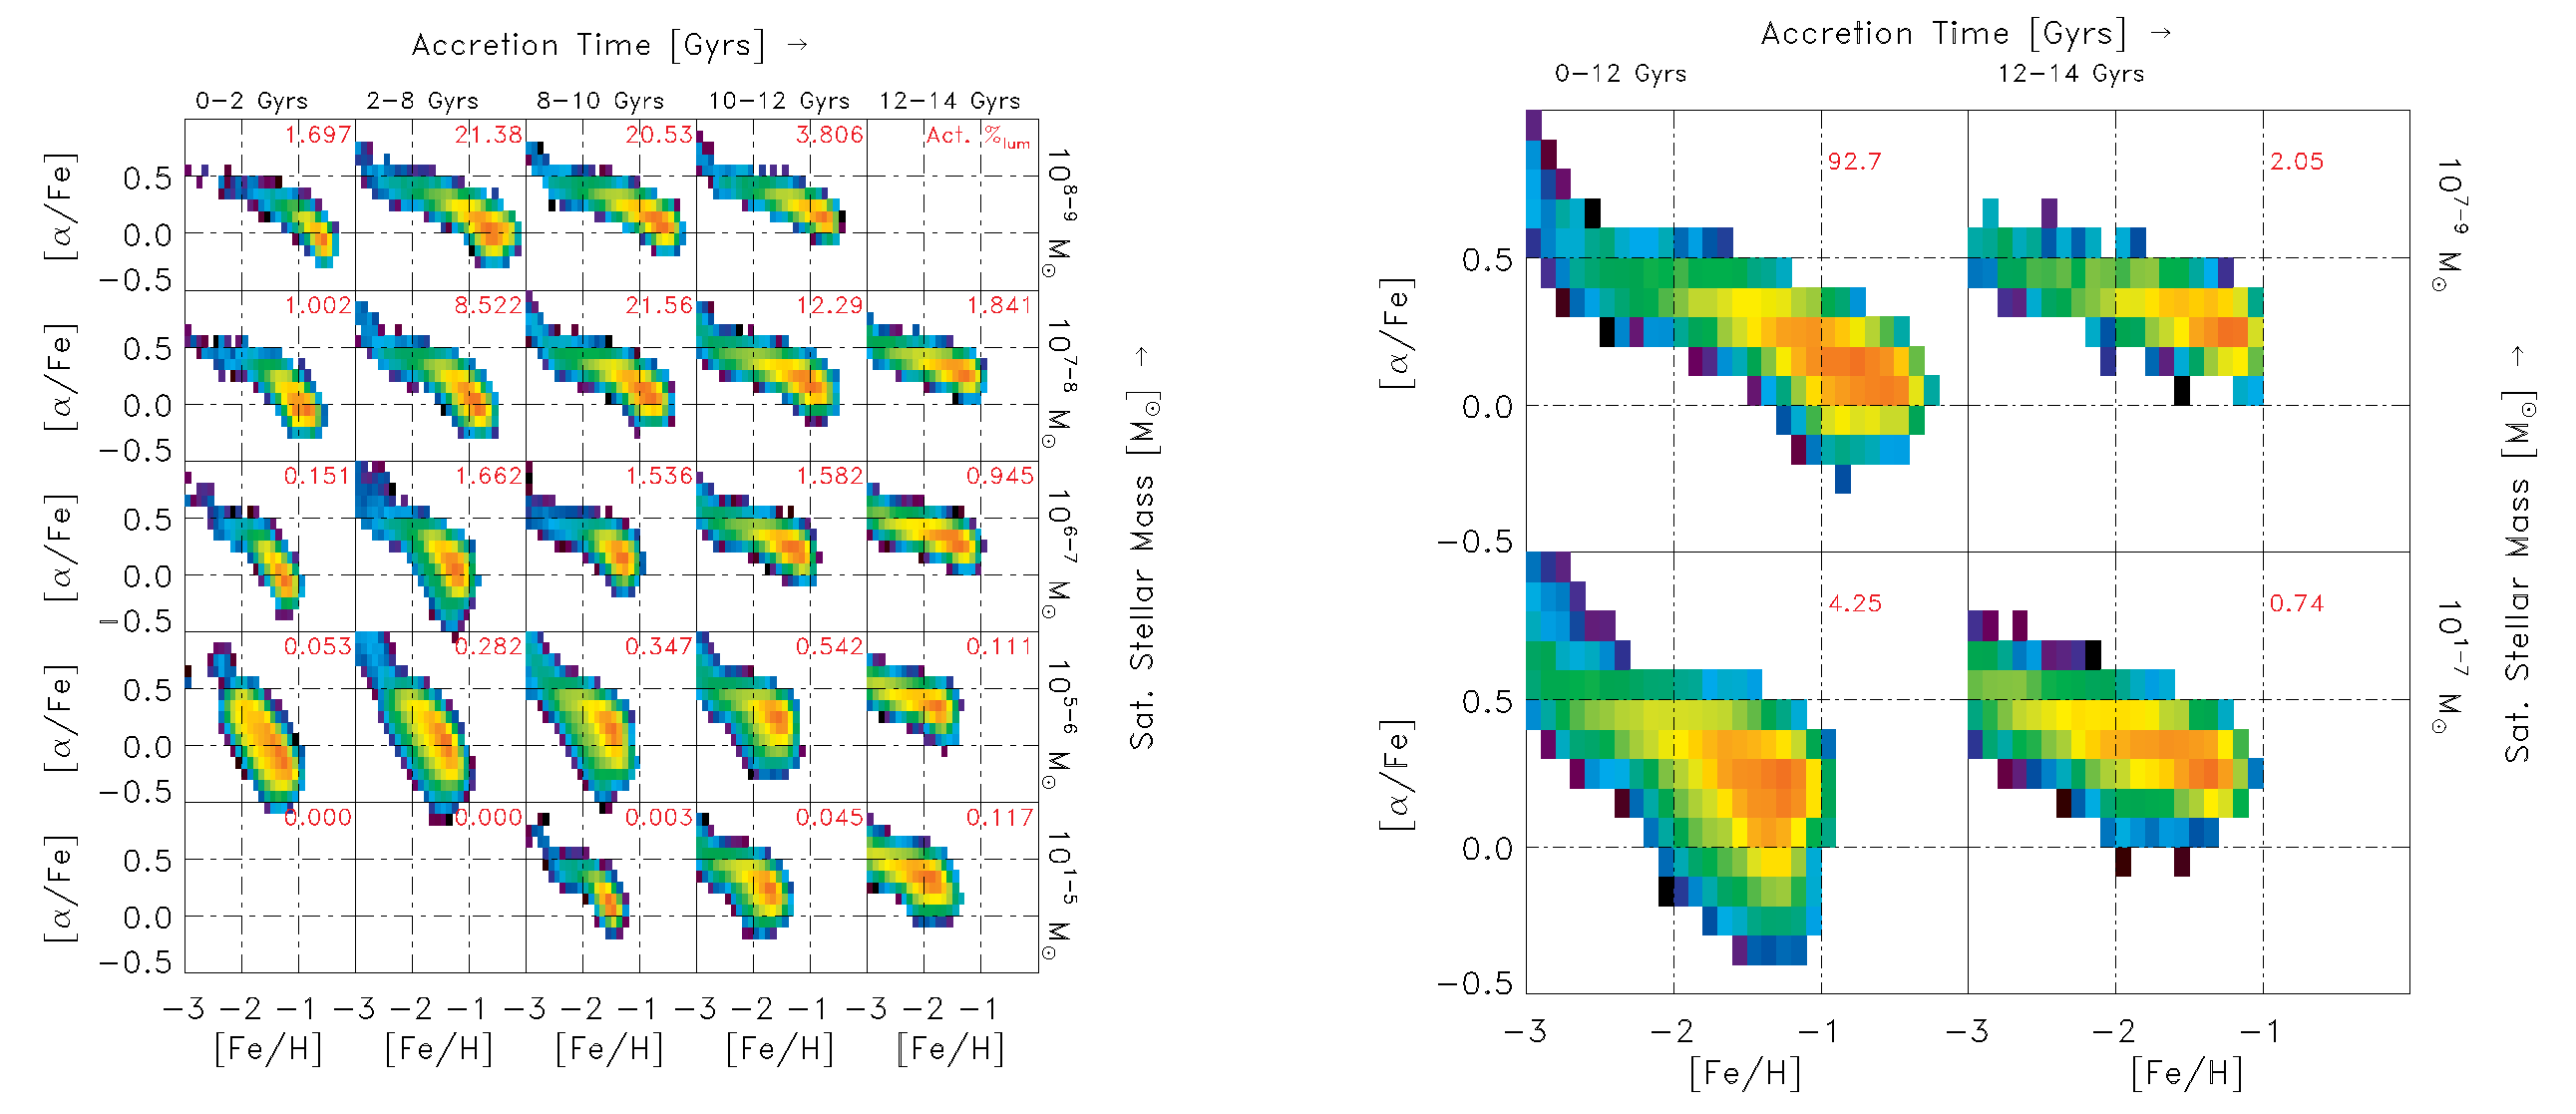
\includegraphics[width=\textwidth]{ourdens.pdf}
			\end{center}
	\end{figure}
	
	
	
	
\end{frame}










%%%%%%%%%%%%%%%%%%%%%%%%%%%%%%%%%%%%%%%%%%%%%%%%%%%%%%%%%%%%%%%
%%%%%%%%%%%%%%%%%%%%%%%%%%%%%%%%%%%%%%%%%%%%%%%%%%%%%%%%%%%%%%%
\begin{frame}{EM formation history for $m$=25}
	
	\begin{figure}
			\begin{center}
				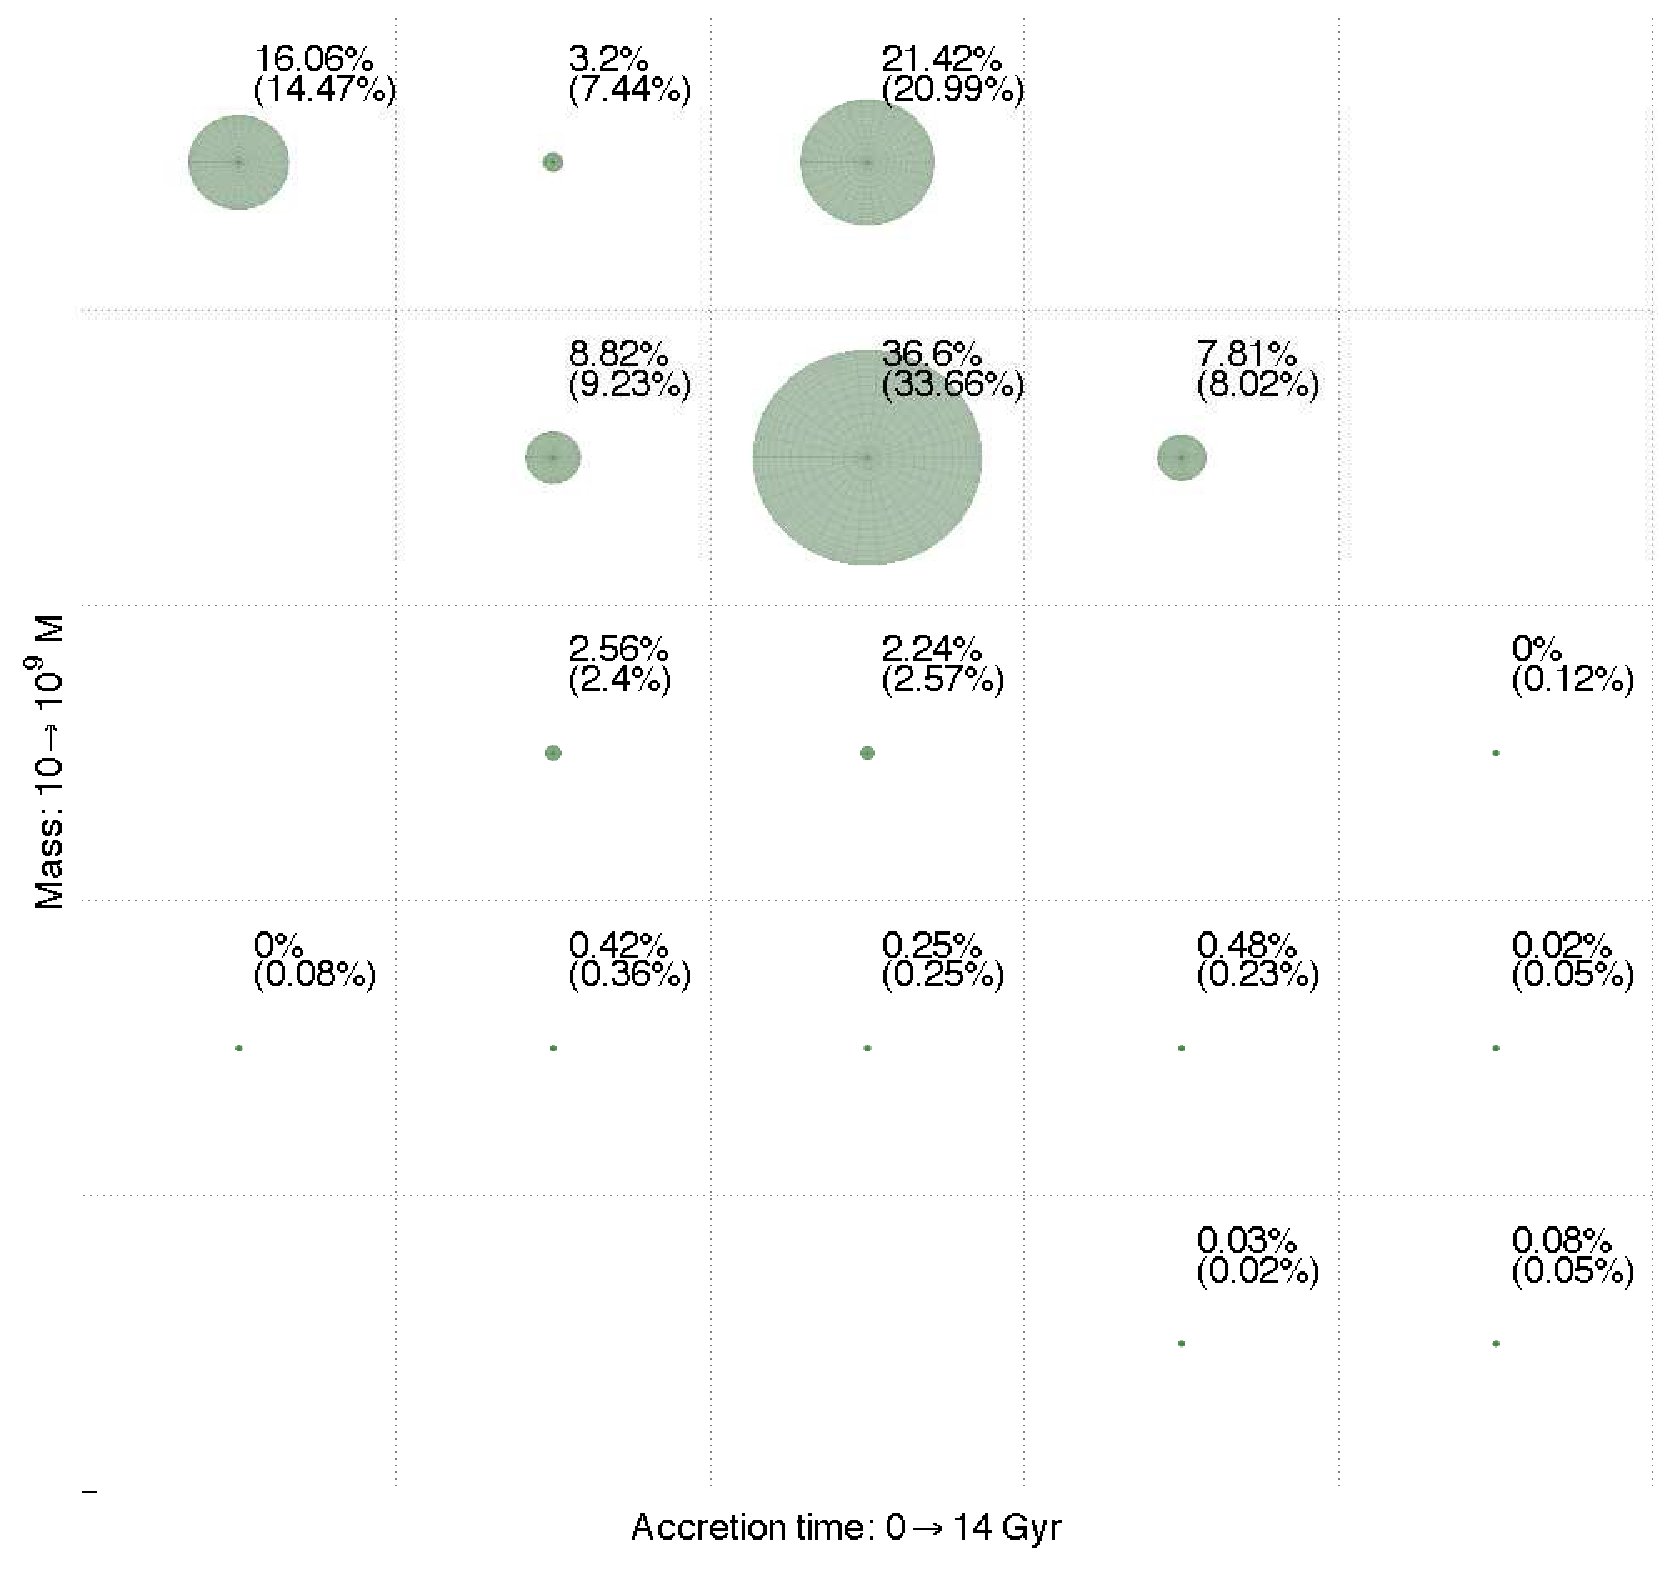
\includegraphics[scale=0.3]{h3fh.pdf}
			\end{center}
	\end{figure}
	
\end{frame}












%%%%%%%%%%%%%%%%%%%%%%%%%%%%%%%%%%%%%%%%%%%%%%%%%%%%%%%%%%%%%%%
%%%%%%%%%%%%%%%%%%%%%%%%%%%%%%%%%%%%%%%%%%%%%%%%%%%%%%%%%%%%%%%
\begin{frame}{EM formation history for $m$=4}
	
	\begin{figure}
			\begin{center}
				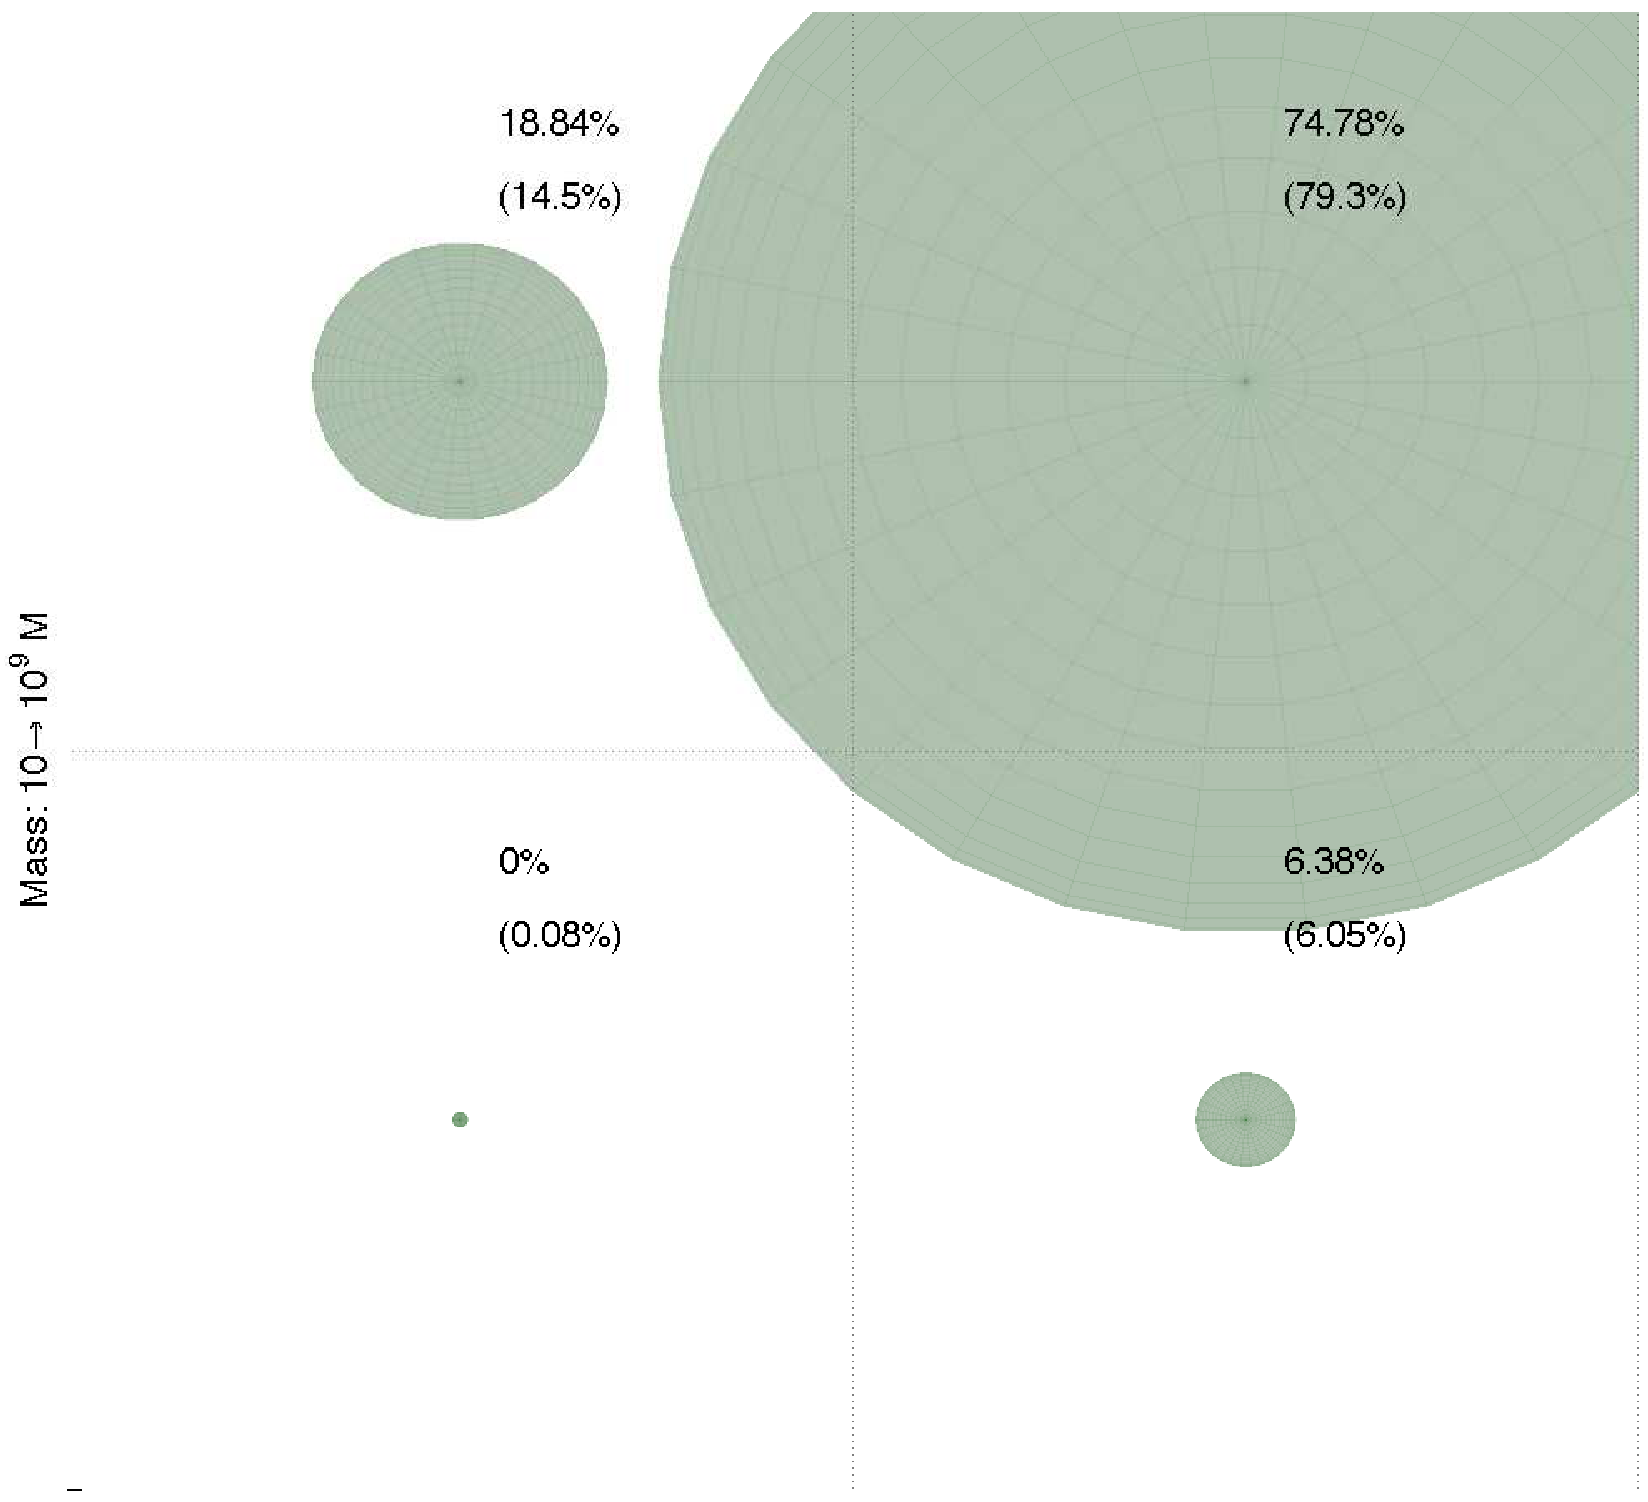
\includegraphics[scale=0.3]{fh2x2.pdf}
			\end{center}
	\end{figure}

	
\end{frame}








%%%%%%%%%%%%%%%%%%%%%%%%%%%%%%%%%%%%%%%%%%%%%%%%%%%%%%%%%%%%%%%
%%%%%%%%%%%%%%%%%%%%%%%%%%%%%%%%%%%%%%%%%%%%%%%%%%%%%%%%%%%%%%%
\begin{frame}{EM overview}
	
	\begin{figure}
			\begin{center}
				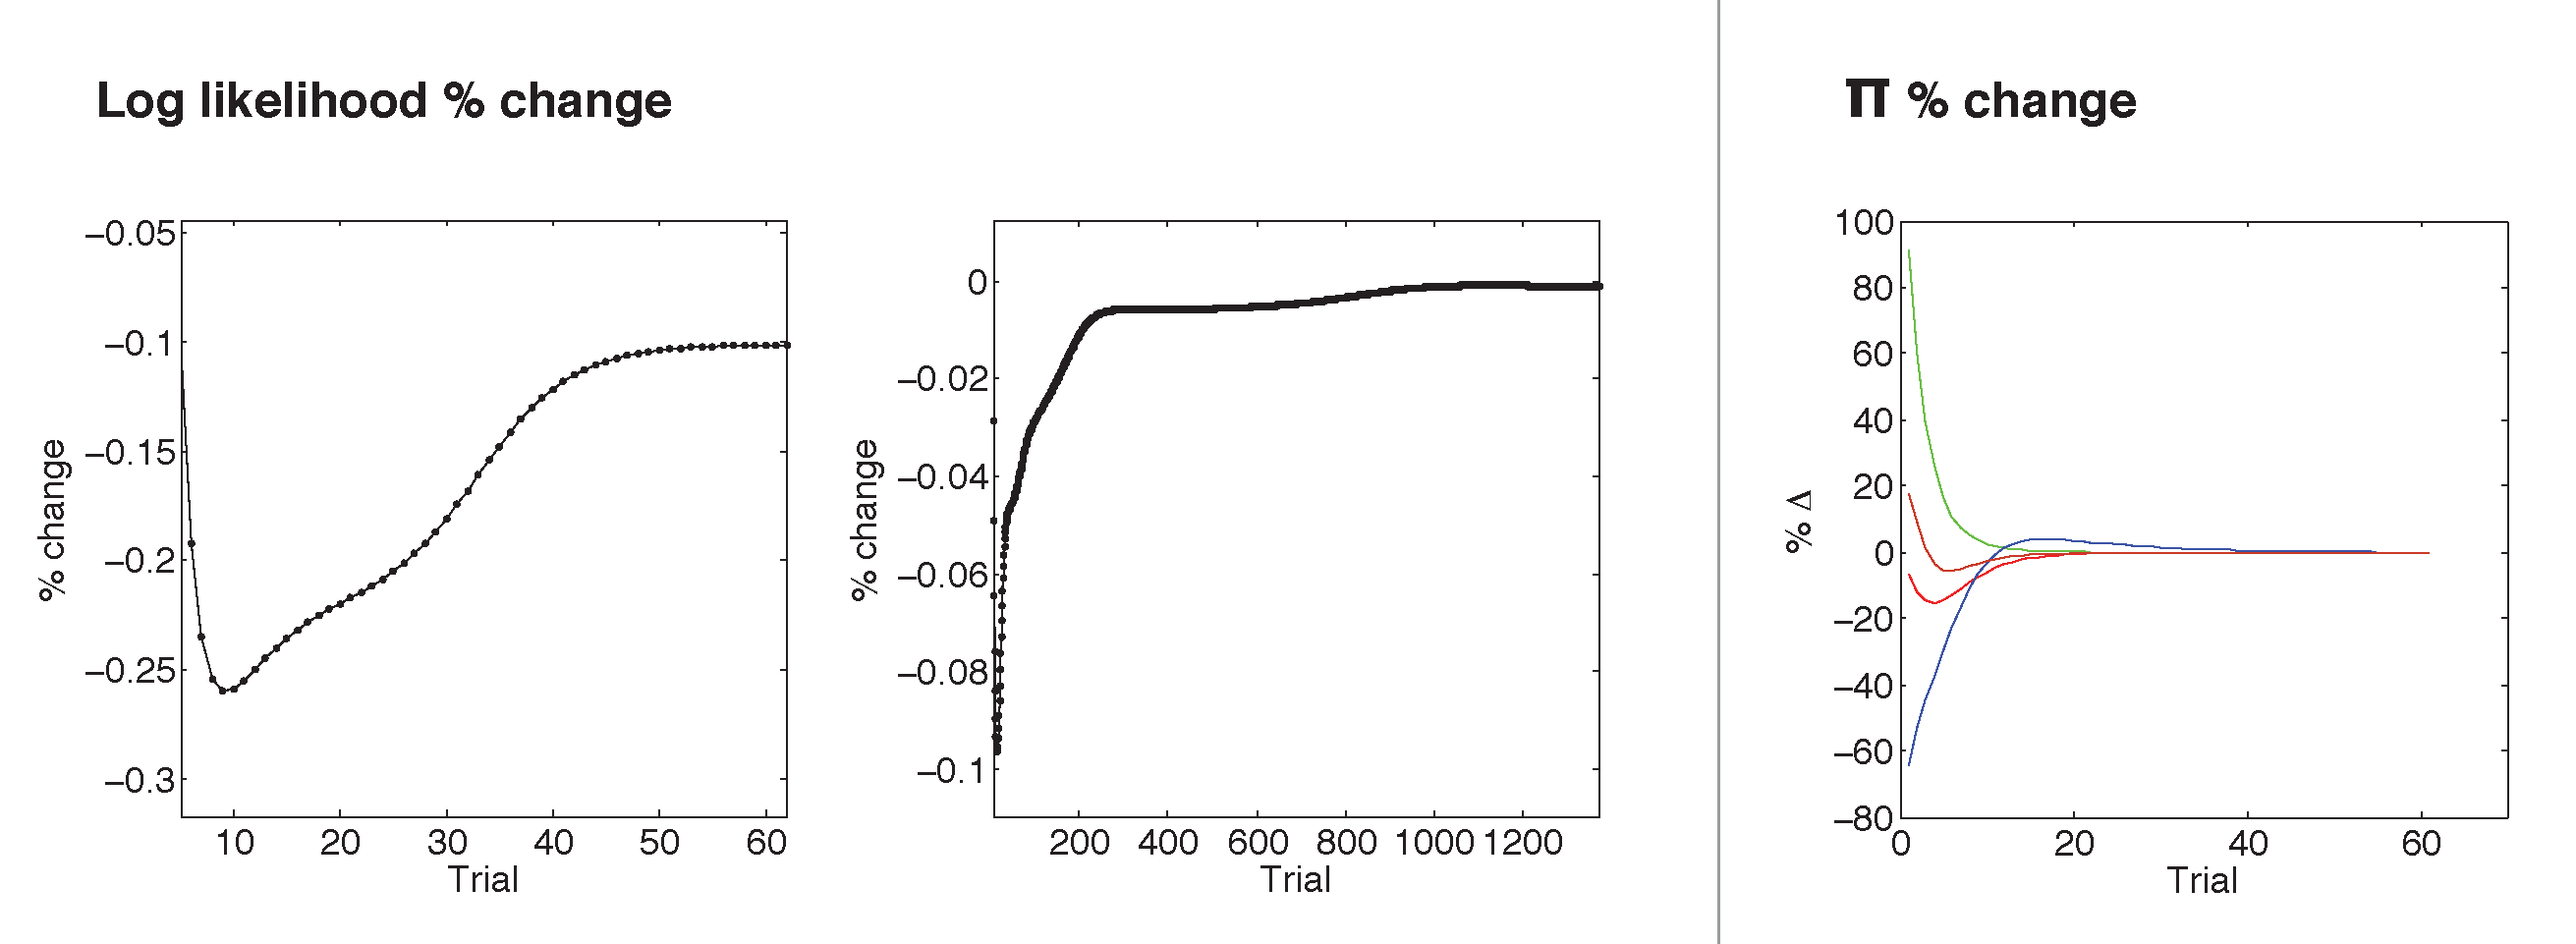
\includegraphics[width=\textwidth]{diag_simple.pdf}
			\end{center}
	\end{figure}
	
	\begin{itemize}
		\item Works with as few as 1,000 observations
		\item Insensitive to initialization of $\vect{\pi}$
		\item Always converges
		\item Large weights identified after 10 iterations
		\item $\llp$ stops changing appreciably after 60 ($m$=4) or 600 ($m$=25) iterations
	\end{itemize}
	
%	1,000 obs, 62 runs, 0.3s m=4
	
%	50,000 obs, 1371 runs, 460s, m=25
	
\end{frame}











%%%%%%%%%%%%%%%%%%%%%%%%%%%%%%%%%%%%%%%%%%%%%%%%%%%%%%%%%%%%%%%
%%%%%%%%%%%%%%%%%%%%%%%%%%%%%%%%%%%%%%%%%%%%%%%%%%%%%%%%%%%%%%%
\begin{frame}{Confidence intervals from observed Fisher Information}
	
	\begin{figure}
			\begin{center}
				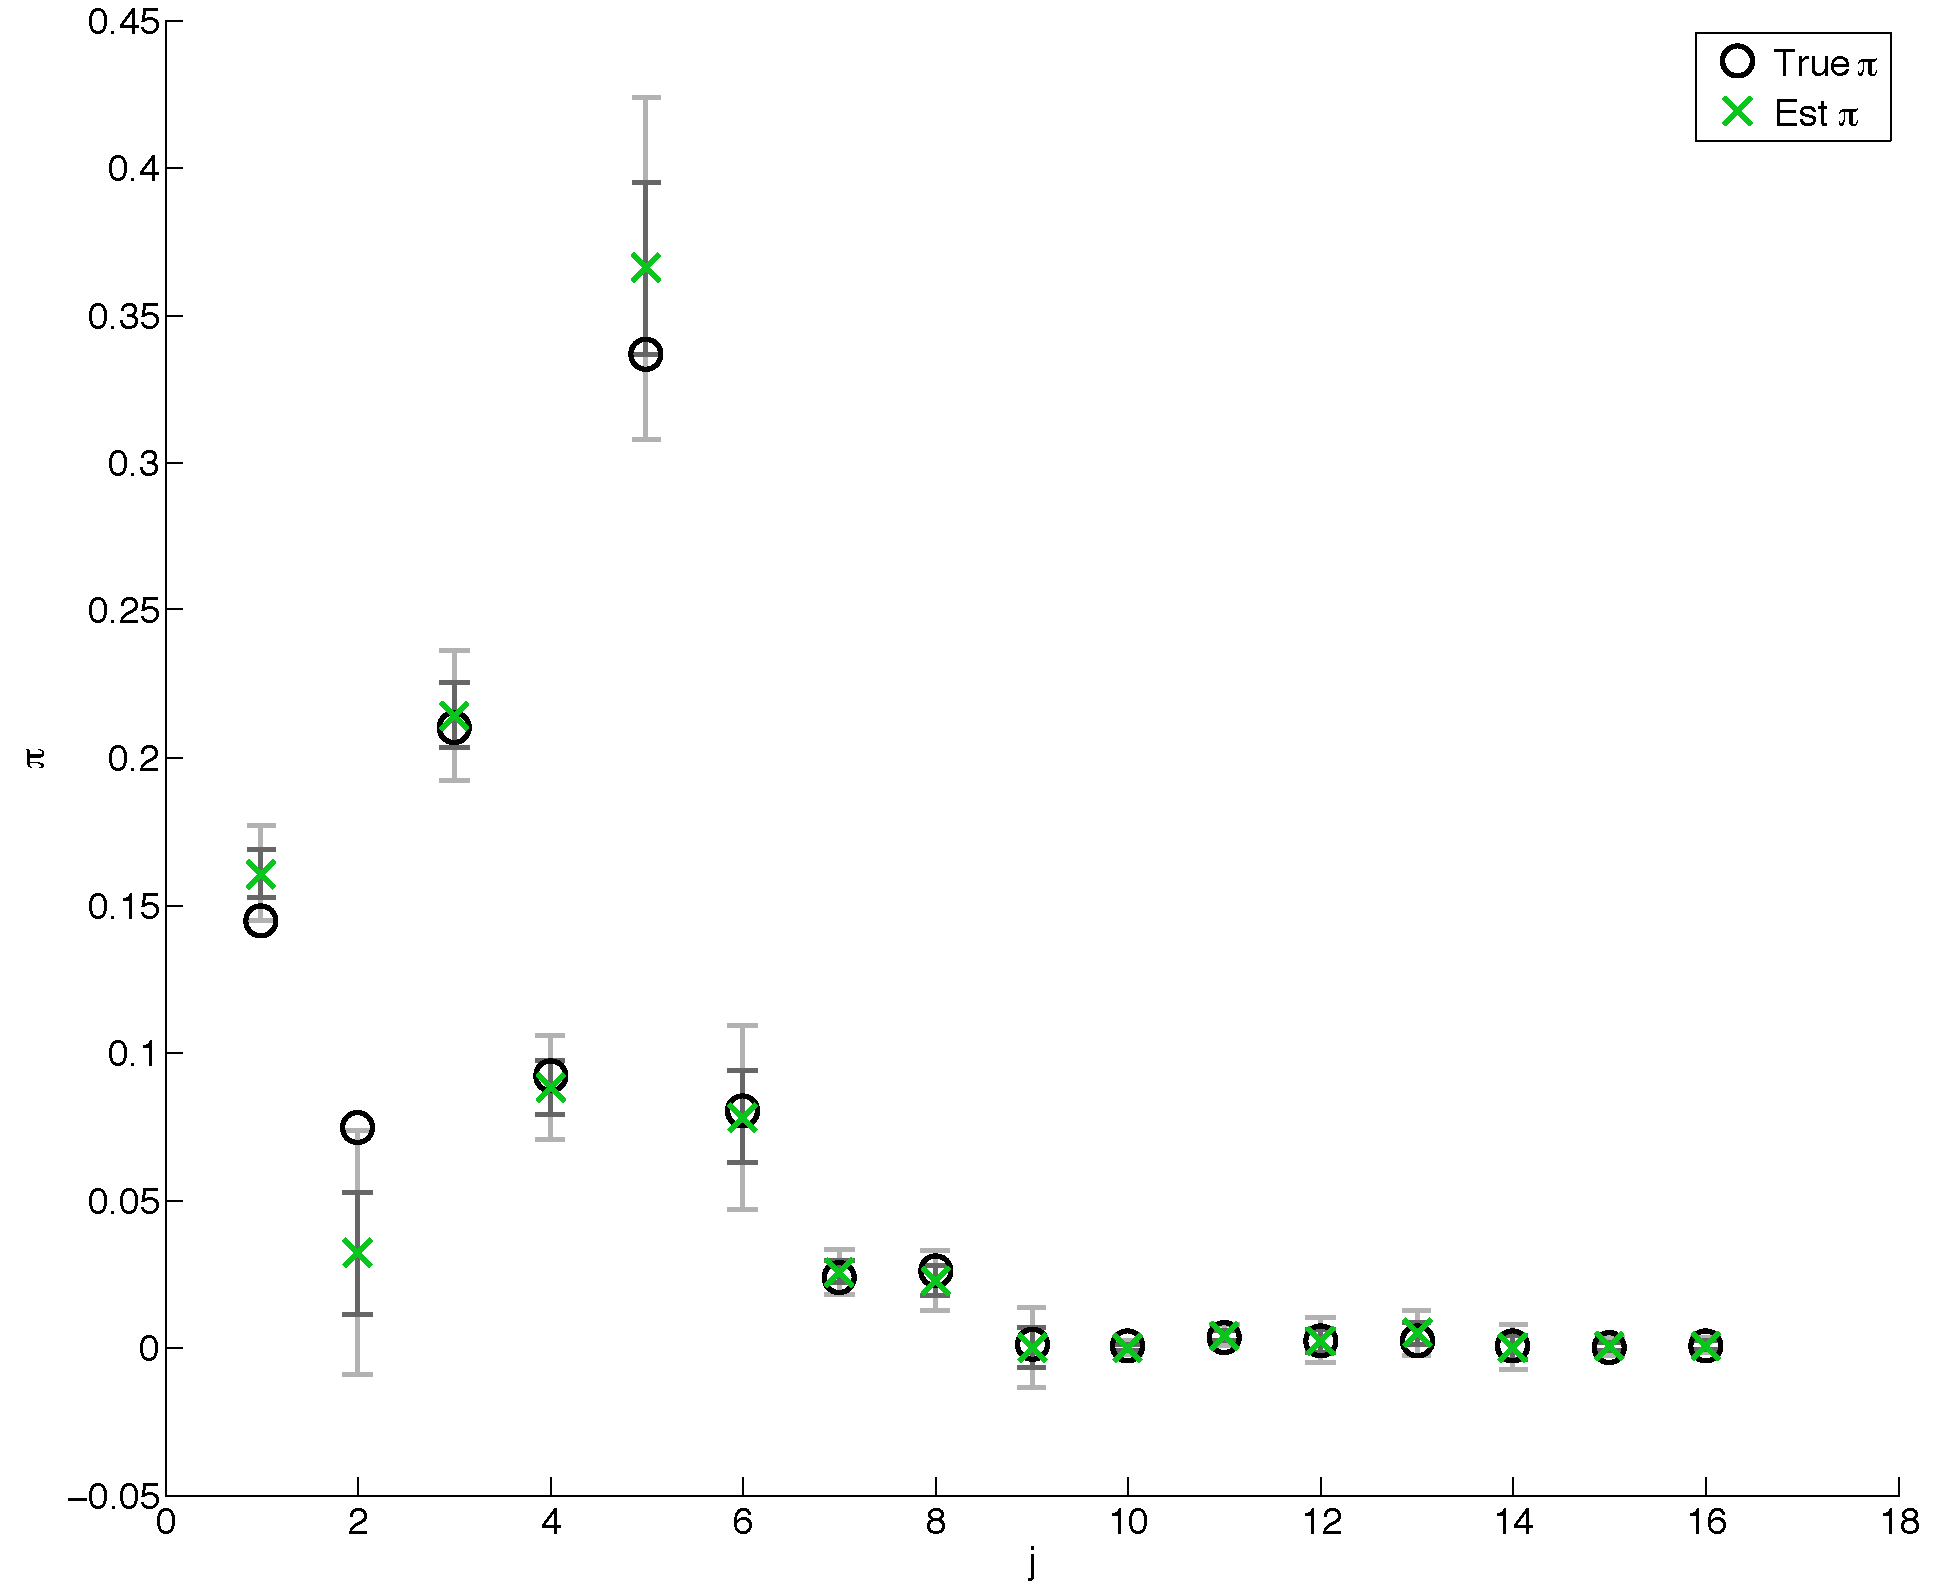
\includegraphics[scale=0.3]{5x5eb.pdf}
			\end{center}
	\end{figure}
	
\end{frame}













%%%%%%%%%%%%%%%%%%%%%%%%%%%%%%%%%%%%%%%%%%%%%%%%%%%%%%%%%%%%%%%
%%%%%%%%%%%%%%%%%%%%%%%%%%%%%%%%%%%%%%%%%%%%%%%%%%%%%%%%%%%%%%%
\begin{frame}{Confidence intervals from observed Fisher Information}
	
	\begin{figure}
			\begin{center}
				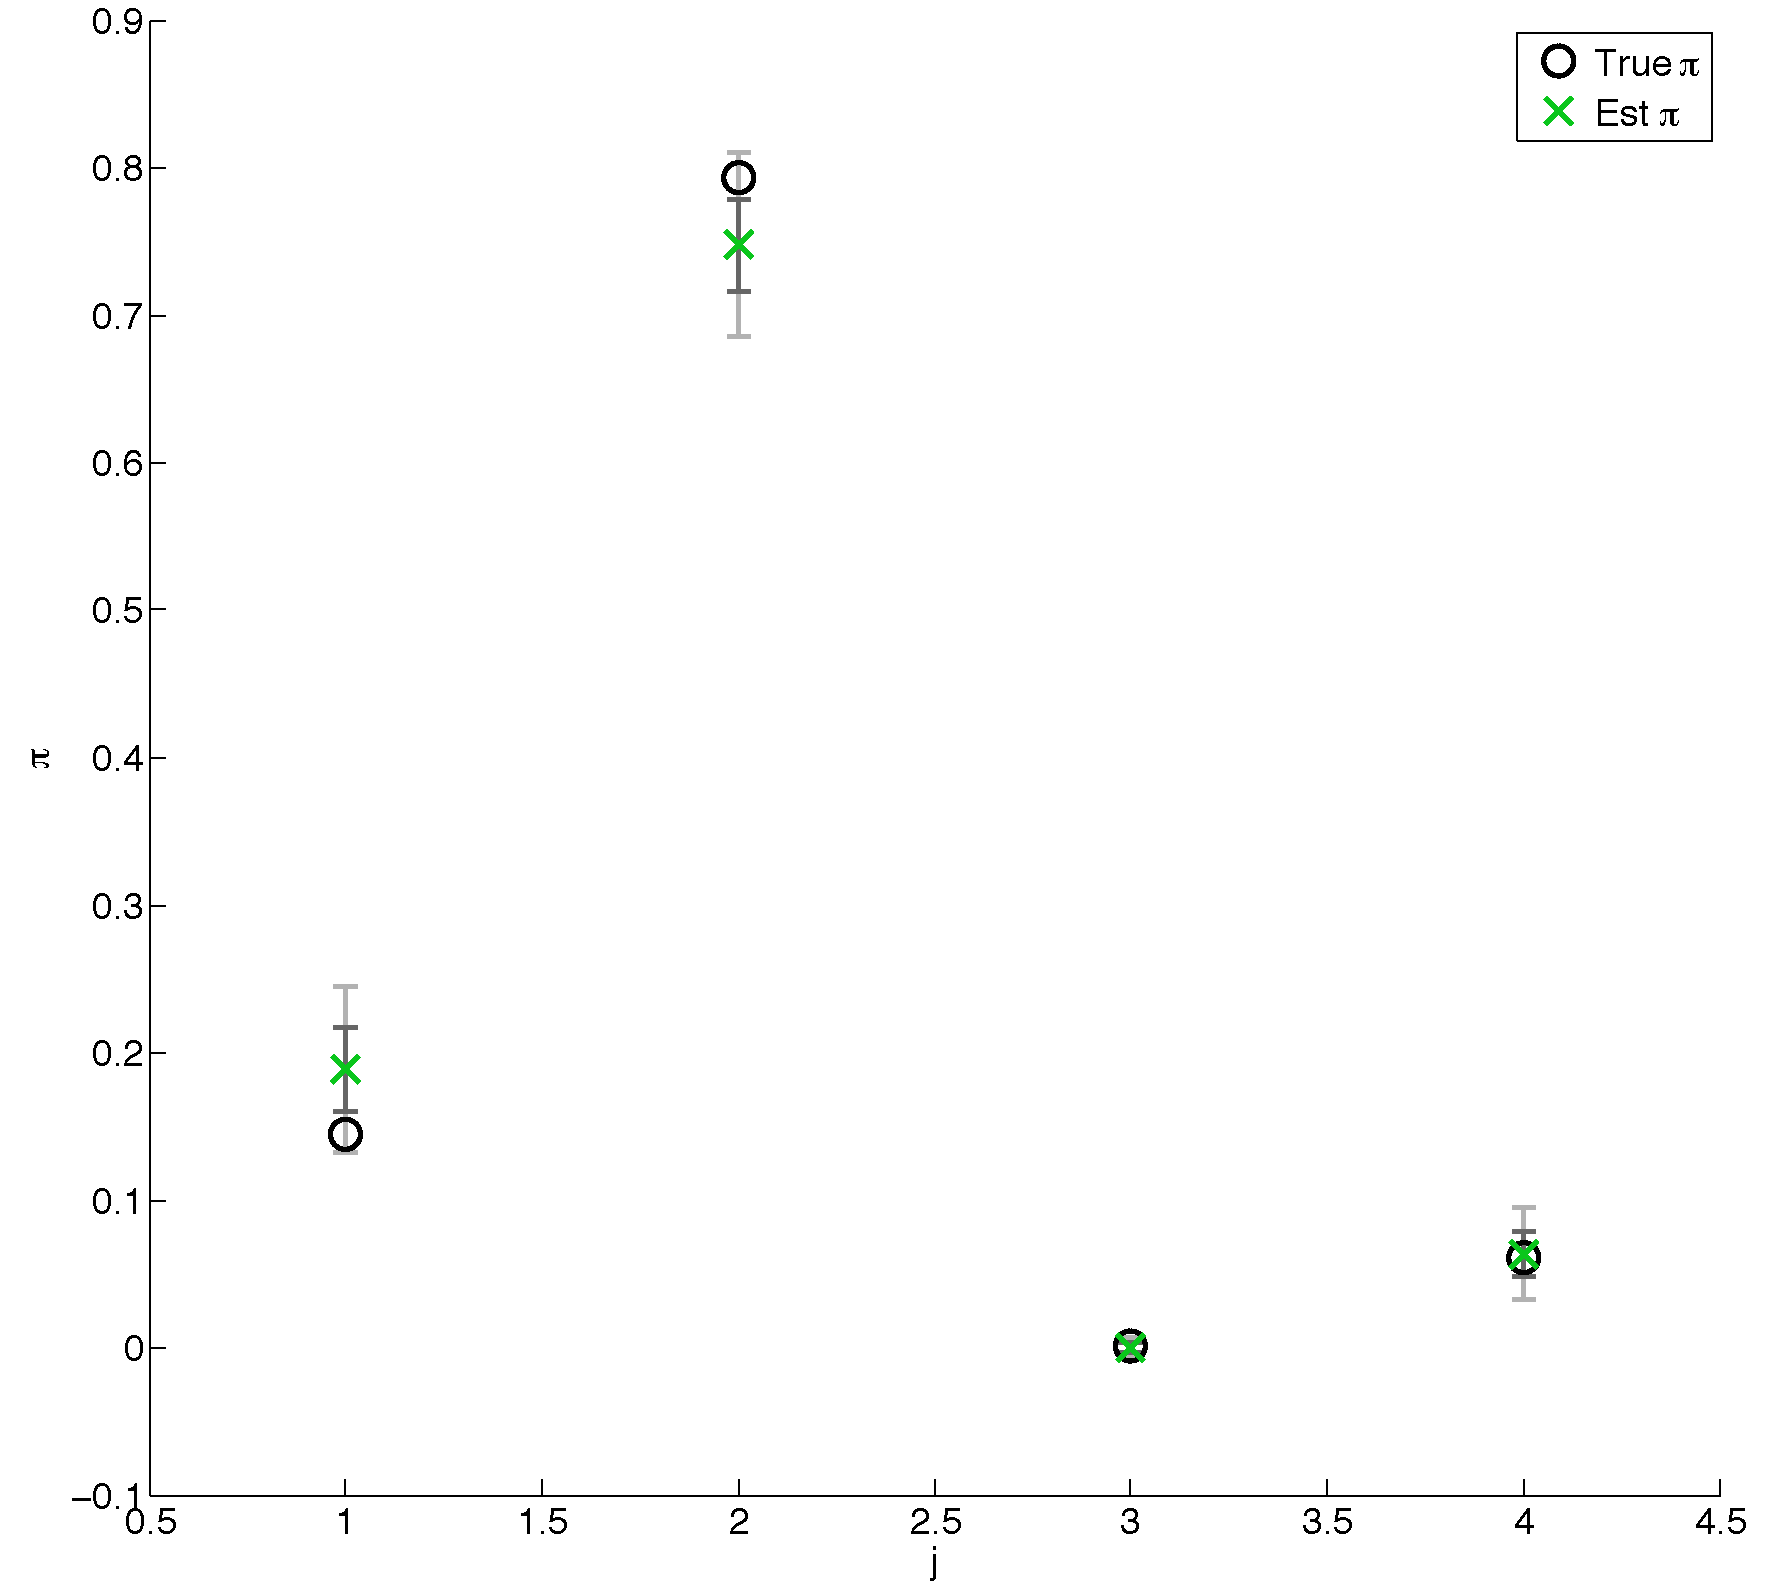
\includegraphics[scale=0.3]{2x2eb.pdf}
			\end{center}
	\end{figure}
	
\end{frame}
















%%%%%%%%%%%%%%%%%%%%%%%%%%%%%%%%%%%%%%%%%%%%%%%%%%%%%%%%%%%%%%%
%%%%%%%%%%%%%%%%%%%%%%%%%%%%%%%%%%%%%%%%%%%%%%%%%%%%%%%%%%%%%%%
\begin{frame}{Correlation between $\vp$}
	
	\eqn{	
		I(\vpg|\vx,\vy)=-\frac{\partial^2 \llpp}{\partial \vp^\prime \partial \vp^{\prime T}}
	}		
	
	\begin{figure}
			\begin{center}
				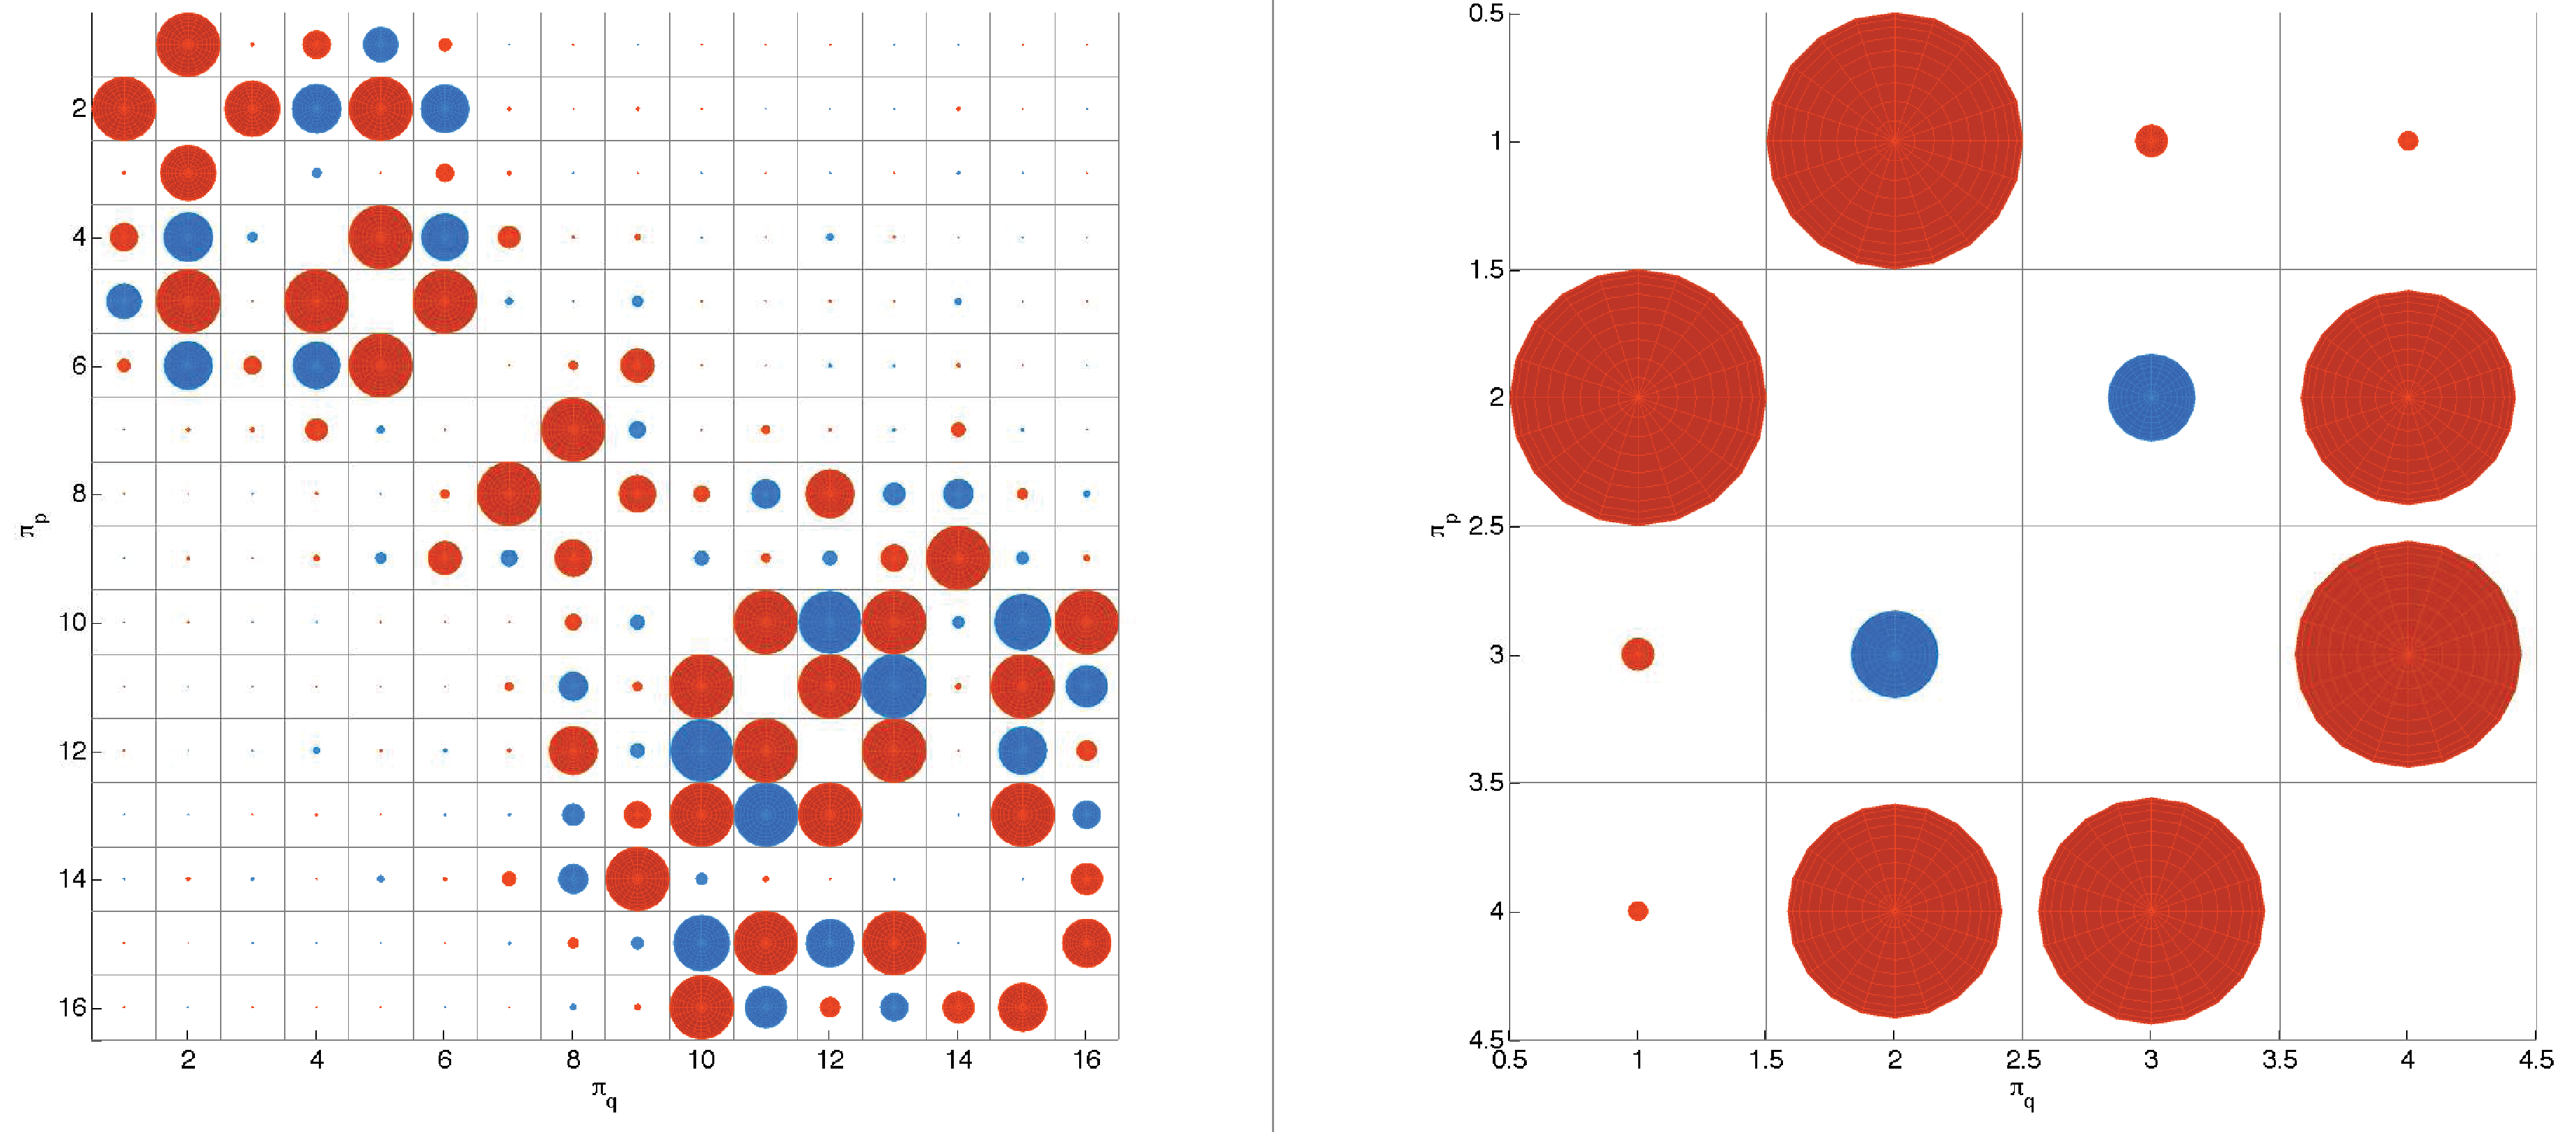
\includegraphics[width=\textwidth]{correl.pdf}
			\end{center}
	\end{figure}	
	
\end{frame}













%%%%%%%%%%%%%%%%%%%%%%%%%%%%%%%%%%%%%%%%%%%%%%%%%%%%%%%%%%%%%%%
%%%%%%%%%%%%%%%%%%%%%%%%%%%%%%%%%%%%%%%%%%%%%%%%%%%%%%%%%%%%%%%
\begin{frame}{Conclusion}
	
	Worked
	\begin{itemize}
		\item 2x2
		\item EM
		\item 5x5 in a few cases
		\item M-of-n bootstrapped errors
	\end{itemize}	
	
	Did not work
	\begin{itemize}
		\item 5x5
		\item Parametric bootstrapped errors
	\end{itemize}	
	
	
	Future improvements
	\begin{itemize}
		\item Non-arbitrary gridding
		\item Smoothing of $f_j$
	\end{itemize}	
	
\end{frame}



































\end{document}


